%%%%%%%%%%%%%%%%%%%%%%%%%%%%%%%%%%%%%%%%%%%%%%%%%%%%%%%%%%%%%%%%%%%%%%%%%%%%
%% Trim Size: 9.75in x 6.5in
%% Text Area: 8in (include Runningheads) x 5in
%% ws-ijwmip.tex   :   26-4-05
%% Tex file to use with ws-ijwmip.cls written in Latex2E.
%% The content, structure, format and layout of this style file is the
%% property of World Scientific Publishing Co. Pte. Ltd.
%% Copyright 1995, 2002 by World Scientific Publishing Co.
%% All rights are reserved.
%%%%%%%%%%%%%%%%%%%%%%%%%%%%%%%%%%%%%%%%%%%%%%%%%%%%%%%%%%%%%%%%%%%%%%%%%%%%
%

%\documentclass[draft]{ws-ijwmip}
\documentclass{ws-ijwmip}
\usepackage{graphicx}
\usepackage[super]{cite}
\usepackage{algorithm, algorithmic}
\usepackage{color}
%\usepackage{split}

\newsavebox\CBox
\def\textBF#1{\sbox\CBox{#1}\resizebox{\wd\CBox}{\ht\CBox}{\textbf{#1}}}
%\parindent=0pt
\newcommand{\RNum}[1]{\uppercase\expandafter{\romannumeral #1\relax}}

% for distanguishing different author emails
\makeatletter
\newcommand{\ssymbol}[1]{\textsuperscript{\@fnsymbol{#1}}}
\makeatother
% for making corresponding author at footnote
\newcommand\blfootnote[1]{%
	\begingroup
	\renewcommand\thefootnote{}\footnote{#1}%
	\addtocounter{footnote}{-1}%
	\endgroup
}

\begin{document}

\markboth{Lina Yang, Hailong Su et al.}{
	Hyperspectral Image Classification Using Wavelet Transform-Based Smooth Ordering 
}

%%%%%%%%%%%%%%%%%%% Publisher's Area please ignore %%%%%%%%%%%%%%%%%%%%%%%
\catchline{}{}{}{}{}
%%%%%%%%%%%%%%%%%%%%%%%%%%%%%%%%%%%%%%%%%%%%%%%%%%%%%%%%%%%%%%%%%%%%%%%%%%

\title{Hyperspectral Image Classification Using Wavelet Transform-Based Smooth Ordering}

\author{Lina Yang\ssymbol{2}, Hailong Su\thanks{Corresponding author}, Cheng Zhong\ssymbol{3}, and Zuqiang Meng\ssymbol{4}}

\address{School of Computer, Electronics and Information, Guangxi University, Nanning, 530004, China\,\\
\email{\ssymbol{2}linayang@gxu.edu.cn\\
	\ssymbol{1}hailongsu@outlook.com\\
	\ssymbol{3}chzhong@gxu.edu.cn\\
	\ssymbol{4}zqmeng@126.com}
}

\author{Huiwu Luo}% \vspace{-7pt}  $^\P$

\address{AI Research, Sichuan Changhong Electric Co.,Ltd., Chengdu, 610000, China\,\\
	\email{luohuiwu@gmail.com}
}

\author{Xichun Li}

\address{Guangxi Normal University for Nationalities, Chongzuo, 532200, China\\
	\email{xichunli@yahoo.com}
}


\author{Yuan Yan Tang}

\address{Faculty of Science and Technology, University of Macau, Macau, 999078, China\\
\email{yytang@umac.mo}
}

\author{Yang Lu}

\address{Department of Computer Science, Hong Kong Baptist University, Hongkong, 999077, China\\
\email{lylylytc@gmail.com}
}

\maketitle

%\begin{history}
%\received{(Day Month Year)}
%\revised{(Day Month Year)}
%\accepted{(Day Month Year)}
%\published{(Day Month Year)}
%%\comby{(xxxxxxxxxx)}
%\end{history}

\begin{abstract}
   To efficiently improve the accuracy of hyperspectral image (HSI) classification, the spatial information is usually fused with spectral information so that the classification performance can be enhanced. 
   To effectively alleviate the general HSI classification problem, in this paper, we propose a new classification method called \textit{wavelet transform-based smooth ordering} (WTSO). Specifically, WTSO consists of three main parts: wavelet decomposition, smooth ordering, and one-dimensional (1-D) interpolation. 
   In this approach, the wavelet transform is firstly imposed to decompose the HSI signal into approximate coefficients (ACs) and details coefficients (DCs). Then, smooth ordering is applied to the ACs so that the coefficients is aligned in a 1-D space. In this procedure, the spatial information is encoded.
   Finally, the simple 1-D signal interpolation tool is adopted to build the final classifier.
   The use of wavelet transform in WTSO is to reduce the high dimensionality of HSI on one hand and capture the intrinsic property of each input signal on the other hand.
   Besides, by converting the hight dimensional samples into a 1-D ordering sequence, WTSO can reduce the computational cost and simultaneously perform prediction for the samples without labels.
   Note that in WTSO, the smooth ordering and 1-D interpolation are used in an iterative manner, and will be terminated after a finite number.
   The proposed method is experimentally demonstrated on two real HSI data sets: IndianPines and University of Pavia, achieving promising results.
\end{abstract}

\keywords{Wavelet transform; smooth ordering; HSI classification; smooth interpolation; feature extraction.}

\ccode{AMS Subject Classification: 22E46, 53C35, 57S20}

\section{Introduction}
Over the past few decades, hyperspectral image (HSI), which is captured through remote sensing sensor, 
has become a hot topic in HSI research community \cite{3}.
A typical hyperspectral image has hundreds of narrow contiguous bands. 
Each pixel is a continuous spectrum that distinguishes different materials. 
Thus, it can be used for recognizing different ground objects with great accuracy and high precision \cite{1,2,4}. 
The object of HSI classification is to assign a meaningful label to each pixel so that the pixel is interpretable.
%However, HSI classification
Although many methods have been developed and proposed to deal with this problem, 
the high similarity of different HSI classes bring many challenges to HSI classification.   
%there are still many , 
These challenges include high dimensionality and small sample size, which is also called \textit{the curse of dimensionality} (``\textit{Hughes phenomenon}''). 
Note that this problem is a normal phenomenon in HSI classification \cite{5}.
%, which leads to a low accuracy .

In order to achieve high classification accuracy, many methods have been proposed \cite{6}. 
Among these methods, support vector machine (SVM) performs state-of-the-art results. 
The strategy of SVM is to map the nonlinear separable data into a much higher dimensional space using a kernel trick, thus that the data can be linearly separated in the kernel-induced space \cite{7,8,9}.
Recently, sparse representation (SR), which was mainly used to process signal data, has been derived and applied to  
%has also been applied in 
HSI classification. 
According to those technical reports published in recent years, SR-based classification methods can obtain excellent classification results \cite{13,14,15,16,17}.
Specifically, the idea of using SR for HSI classification was first introduced by Chen {\it et al.} \cite{18}, where their proposed method is named \emph{sparse representation classification} (SRC) method.
According to our understanding, SRC method assumes that HSI pixels can be sparsely represented by a linear combination of a few training samples over a dictionary. 
The solution of this problem can be typically solved by a greedy algorithm, such as orthogonal associated pursuit (OMP) algorithm. 
The final test label is determined by a minimal residual principle.
%The main idea of SVM is  to find a lower space to solve high dimensional problem, then, it can process HSI data conveniently and efficiently.



Note that for HSI classification, the adjacent pixels trend to belong to the same class.
It can serve as a prior knowledge, helping to decide the class label of the test sample.
Thus, the spatial information is very helpful to determine the hardly classified samples.
Motivated by this observation, 
%the spatial information is usually encoded into
many spectral-spatial approaches are proposed \cite{19}.
For example, 
Tang {\it et al.} \cite{20} proposed two kinds of sparse representation algorithms based on manifold to exploit the local structure of a test samples, where the spatial information is encoded as a regularization term in the objective function.
%in corresponding sparse representation for enforcing smoothness across neighbor samples sparse representation.
Luo {\it et al.} \cite{21} proposed a spectral-spatial one-dimensional manifold embedding (SS1DME), which utilizes the spectral-spatial information-based metric to learn the similarity of HSI pixels.
%In this method, the contextual information is encoded via a spectral-spatial metric model. %via spatial information to obtain the promising result

%Besides the classifier, many researchers focus on the feature representation, \textit{i.e.} feature extraction or feature selection.
%models have also been proposed for HSI classification .
%The main theme of these methods is to .
One of the main stream is to reduce the dimension of HSI data without losing the discriminant information \cite{10,11,12}.
Specifically, wavelet transform, which considers the problem in the frequency domain, is a powerful mathematical tool to extract the useful information for classification. 
Given an input signal, it provides time-frequency localization to distinguish different classes \cite{nayak2016brain}.
%Wavelet transform is usually adopted for for dimensionality reduction.
Wavelet transform provides an efficient way to reduce the dimensionality of HSI data.
Considering this advantage, 
many wavelet transform based methods have been introduced for HSI classification. For example, Wang {\it et al.} \cite{22} proposed stationary wavelet transform (SWT) to extract the spatial features. 
Each spectrum band image is firstly converted to SWT domain, then principal component analysis (PCA) is applied to reduce the dimensionality, finally $k$-nearest neighbors algorithm is employed for classification. 
Tang {\it et al.} \cite{24} proposed a 3-D scattering wavelet transform, which filters the HSI cube data with a cascade of wavelet decompositions\cite{25}.
Qian {\it et al.} \cite{29} proposed a method based on structured sparse logistic regression and 3-D discrete wavelet transform (3D-DWT) texture features.
However, the aforementioned methods work on high-dimensional space.
The complex theory makes the decision bound hard to determine.

In order to deal with this issue, Wang \cite{34} proposed a novel method called \emph{smooth ordering} to classify the handwritten digits, achieving comparable results.
Motivated by his pioneered work, in this paper, we try to integrate wavelet transform with smooth ordering to further explore the potential power of smooth ordering.
We point out that our work is similar to the work taken by Ram {\it et al.} \cite{30}. 
According to their publication, their work is highly effective when used in image denoising, inpainting, and deblurring. However, in their work, smooth ordering is applied to overlapped patches, and the input signal is two dimensional, which is not suitable for HSI classification. In order to be able to fit the task of HSI classification, with a slight modification, 
we define a new distance measure before applying the scheme of smooth ordering. 
Then, according to the observation that the ACs contains the main information of the input signal, smooth ordering is applied to ACs only. 
%To do this, we can process the ACs in 1-D space.
%The main idea of this paper explained as follows:


The main steps of our method can be explained as follows:
Firstly, the wavelet transform is adopted to decompose the HSI image into ACs and DCs.
Secondly, using a distance measurement in our previous work \cite{31},
smooth ordering is performed on the ACs, where the dissimilarity of each sample is calculated accordingly.
Next, based on the measurement, smooth ordering algorithm is applied to the coefficients,
%which can be smoothly reordered and further embedded into a 1-D sequence.
resulting in an ordered sequence of these data in 1-D space.
Finally, a group of  classifiers are constructed using 1-D interpolation,
and the final class is assigned by the maximum voting rule.
%which is a simple tool for 1-D signal processing.



The highlight of this work is to explore the capability of smooth ordering in frequency domain using wavelet transform. In details, we refine the following aspects to highlight our preliminary work: 
\begin{enumerate}
\item A new metric is defined to make our algorithm work properly in the wavelet domain. 
\item Smooth ordering is introduced to explicitly find out the decision bound, making the results more intuitive. 
\end{enumerate}
More importantly, the results of WTSO is superior when compared with other state-of-the-art methods.

%
%The main contribution of our proposed method are summarized as follows:
%\begin{romanlist}[(ii)]
% \item A novel method called WTSO is proposed for HSI classification, which processing decompose coefficient in 1-D space.
% \item Using a new distance measure to define smooth ordering.
%\item  Apply smooth ordering to the approximate coefficient, which can be embedded into 1-D sequence.
%\end{romanlist}


The remainder of this paper is organized as follows. The proposed WTSO is described in Section \ref{sec:proposed}. The effectiveness of the proposed WTSO method is experimentally evaluated and discussed in Section \ref{sec:experiment} using two real HSI data sets. Finally, we conclude our work in Section \ref{sec:conclude}.



\section{Methodology}\label{sec:proposed}
\begin{figure}[bh]
	\centerline{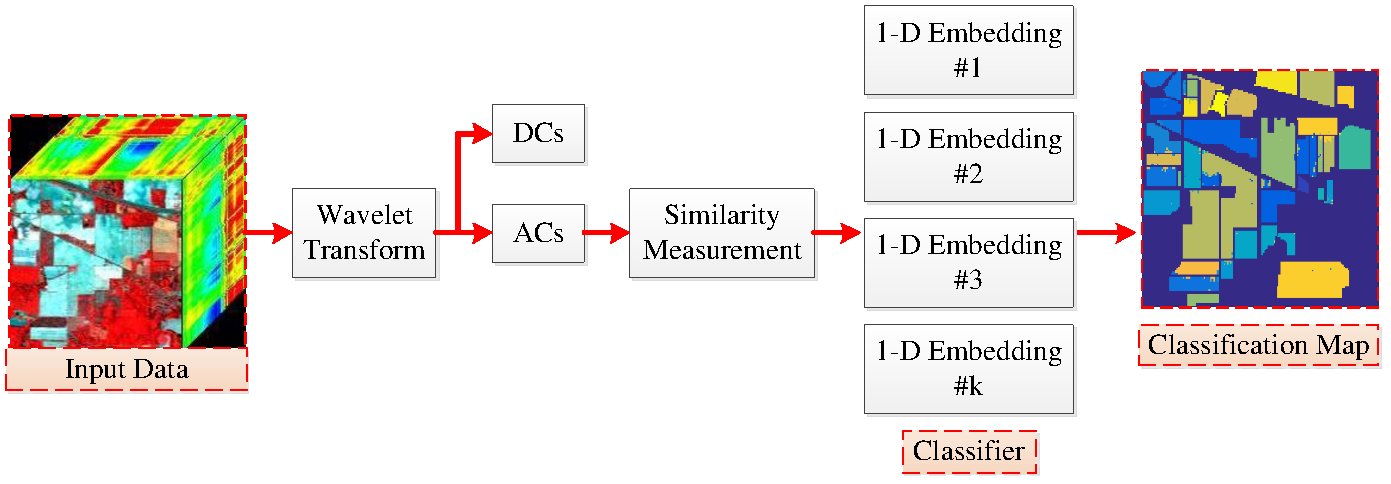
\includegraphics[width=13cm]{image/flow-chart}}
	\vspace*{8pt}
	\caption{Flowchart of the proposed WTSO classification scheme.}
	\label{figure1}
\end{figure}
In this section, we introduce our proposed  WTSO method. The flowchart of our method is shown in Fig. \ref{figure1}.
%, where SO1CB is the abbreviation of the developed smooth ordering-based scheme. %Interpolation uses cubic spline interpolation in our scheme.
The details are described in the following subsections.


\subsection{Descriptive Transformation by Wavelet Decomposition}
In this section, we briefly review the concept of wavelet transform.
Wavelet transform can be found in any articles that are related to the concept of wavelet, such as the one in Qian \textit{et al.} \cite{29}. 
%In mathematics, a wavelet is , which can be used to extract information from many different kinds of data,  processing. 
%Wavelet transform is a  tool for multiresolution analysis. 
%It can analyze different kinds of data, such as 1-D signal data and 2-D image data. 
Wavelets are powerful mathematical tool to analyze 1-D/2-D signal data in time-frequency domain.
An input signal can be decomposed from mother wavelets that are scaled and translated. 
%Mathematically, wavelet transform is defined by:
This procedure can be formalized as: %formulize
\begin{equation}
(W_{\psi f})(a,b) = \;<f(t),\psi _{a,b} (t)>\; = \int f(t)\psi _{a,b} (t)dt
\label{equ2.1}
\end{equation}
where $\psi_{a,b}(t) = (1/\sqrt{|a|})\psi_{(t-b/{a})}$, and $\int \psi (t)dt=0$. 
%The symbol $<\cdot>$ is an inner product. 
The parameter $a$ is a scale factor that dependently scales the frequency.
Large $| a |$ means low frequency, whereas small $| a|$ means high frequency.
On the other hand, parameter $b$ is the time of input signal. 
%Therefore, wavelet transform can analysis signal in time and frequency domain. 


Benefiting from the two parameters, wavelet transform can observe signal structures by by discreting the parameters $b$ and $a$ (\textit{i.e.}, time and frequency domain).
%If parameter $a$ and $b$ are discrete values, the wavelet transform is called discrete wavelet transform, which defined as follows:
In that case, the \emph{discrete wavelet transform} is obtained:
\begin{equation}
(W_{\psi f})(m,n) 
%W_{m,n}^{\psi } 
=\; < f(t),\psi _{m,n}(t)>\; = \int f(t)\psi _{m,n}(t)dt
\label{equ2.2}
\end{equation}
where $\psi _{m,n}(t)=a_{0}^{-m/2}\psi (t-n{b_0}{a _{0}^{m}}/{a _{0}^{m}})$.
Using discrete wavelet transform, the signal is decomposed into approximate coefficients (ACs) and detail coefficients (DCs), respectively. 

If the wavelet functions and scaling functions are symbolized by $\psi(t)$ and $\varphi(t)$, the original signal $f(t)$ can be recovered by:
\begin{equation}
f(t)=\sum _k c_{j_0}(k)\varphi _{j_0,k}(t) + \sum_{j=j_0}^{\infty }\sum _k d_j(k)\psi _{j,k}(t)
\label{equ2.3}
\end{equation}
where the ACs $c_{j_0,k}$ and DCs $d_{j,k}$ are given by:
\begin{equation}
c_{j_0,k} =\; < f(t),\varphi _{j_0,k}(t)>\; =\int f(t) \varphi _{j_0,k}(t)dt
\label{equ2.4}
\end{equation}

\begin{equation}
d_{j,k} =\; < f(t),\psi _{j,k}(t)>\; =\int f(t) \psi _{j,k}(t)dt
\label{equ2.5}
\end{equation}

In the proposed WTSO approach, we use a 2-D discrete wavelet transform to extract the descriptive features that are stored in the decomposed coefficients.
Particularly, the symlets wavelet, which is a modified version of Daubechies wavelets by increasing the symmetry, is adopted. 
%After decomposing the image, we obtain the ACs and the DCs, respectively. 
Because the information of an image is mainly represented in the ACs, we only use the approximate coefficients. The demonstration is visualized in Fig. \ref{figure2}. 

\begin{figure}[htb]
	\centerline{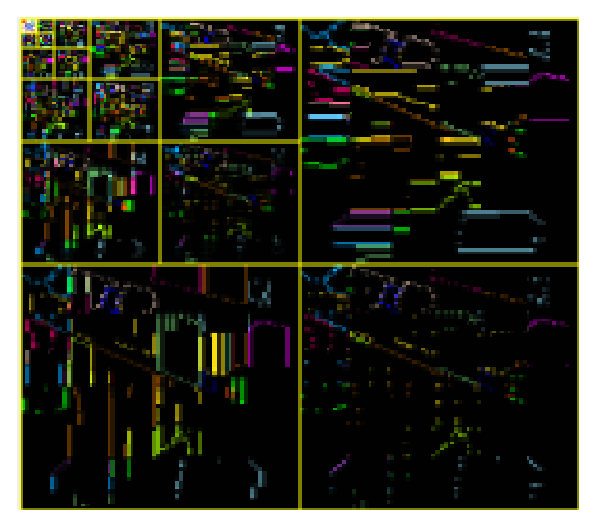
\includegraphics[width=6cm]{image/decompose}}
	\vspace*{8pt}
	\caption{
		A graphical demonstration of Wavelet decomposition using Indian Pines image
		%The wavelet decompose of the Indian Pines image as an example 
		(The decompose level is 5).
	}
	\label{figure2}
\end{figure}



\subsection{Smooth Ordering of Input Signals}
%{Obtaining Descriptive Features by Wavelet transform}
%


%\subsubsection{Decomposition scheme}
Let $\mathcal{X}=\{x_i\}_{i=1}^N\in \mathbb{R}^n$ be a set of HSI pixels which are choose from $M$ different classes. The data set $\mathcal{X}$ can be expressed as a matrix $X = [x_1,x_2,x_3,\dots,x_N] \in \mathbb{R}^{n\times N}$, where each column stands for a pixel in $\mathcal{X}$. The notation $\mathcal{Y} \in \{1,2,\dots,M\}$ is the set of class labels. 


%Once the ACs of an HSI image is given, smooth ordering is used to produced smooth coefficients . Next section we expound how to achieve a smooth coefficients of HSI.
%\subsection{Building the smooth coefficients}

The goal of smooth ordering is to design an operator that is applied to approximate the coefficients and produces an ordering under the given distance metric. 
%To continue our discussion, we  
%assume that 
%Under the given metric, 
%two similar pixels means that their approximate coefficients are also similar.
In the new ordering, pixels with similar spectral signature should be stay as close as possible.

In our previous work \cite{31}, we proposed a spectral-spatial distance measure for smooth ordering. The quality of distance measurement is very critical for improving classification accuracy \cite{ML1DE}. Here, a new distance measurement is developed to measure the similarity of different samples. 

The spectral distance $D^w(a_i, a_j)$ between samples $x_i$ and $x_j$ is defined by:
 \begin{equation}
    D^w(a_i, a_j) = 1 - exp(-\frac{\left \| x_i - x_j \right \|^2}{\rho _i\rho _j})
    \label{equ2.6}
\end{equation}
 where $a_i\in \mathcal{S}=\{1,\cdots, N\}$ is the index of the $a_i$-th sample in $\mathcal{X}$, and 
 $\rho_i$ is a local scaling parameter defined by:
 \begin{equation}
   \rho _i = \left \| x_i-x_i^{K_{nn}} \right \|.
   \label{equ2.7}
\end{equation}
Here,  $x_i^{K_{nn}}$ is the $K_{nn}$-th neighbor around $x_i$, and $\left \| * \right \|$ is a $l_2$ norm.

In order to improve classification accuracy, the spatial distance between two samples $x_i$ and $x_j$ is encoded according the the following equation:
 \begin{equation}
  D^s(a_i,a_j) =\left\{\begin{matrix}
-\mu, & \mbox{if} \;j \in {\omega_i}.\\
0,  & otherwise
\end{matrix}\right.
 \label{equ2.8}
\end{equation}
where $\mu > 0$ is a weighing parameter that is used to enhance the similarity using a spatial prior. The symbol of $\omega_i$ is defined by:

 \begin{equation}
  \omega _i = \{j\in \mathcal{S} \mid dist(x_m, x_n) \leqslant \sqrt{r}\}
   \label{equ2.9}
\end{equation}
 where $dist(x_m, x_n)$ is the distance between $x_m$ and $x_n$. $\mathcal{S} = \{1,2,3,\dots,N\}$.
 
 Using the above notations, the spectral-spatial metric is given by:
 %Finally, the distance measure is defined as follows:
  \begin{equation}
  D^{ws}(a_i, a_j) = D^w(a_i, a_j) + D^s(a_i, a_j).
   \label{equ2.10}
\end{equation}

%Under this distance measure, 
In fact, smooth ordering operated on the sequences $\{a_i\}_i^N$ can be considered as a permutation $P$ on $A=[a_1, \cdots, a_N]$, where $a_i \in \mathcal{S}$.
The effect is that all sequences will be reordered into a new sequence $A^P=[a_1^P,a_2^P,a_3^P,\dots,a_N^P]$ ($a_i^P \in \mathcal{S}$). 
Clearly, there are many kinds of such sequences. 
But only the one which has the shortest traveling path is meaningful and closely related to our problem.
Substantially, our problem is a in fact a TSP problem.
Therefore, our problem can be solved by the following optimization:
\begin{equation}
  P = arg \min _P a_{TV}^P, ~~ a_{TV}^P = \sum_{i=1}^{N-1}D^{ws}(a_{i+1}^P,a_i^P).
   \label{equ2.11}
\end{equation}
%where
%
%\begin{equation}
%  a_{TV}^P = \sum_{i=1}^{N-1}D^{ws}(a_{i+1}^P,a_i^P).
%   \label{equ2.12}
%\end{equation}

%Therefore, the shortest path is obtained that through the set of $a_i$. This can be regarded as a traveling salesman problem (TSP), which is become computationally and effectively for large sets.

%We defined $\pi$ is a permutation of the index $S = \{1,2,3\dots ,N\}$, that is $a_{\pi(i)} = a_i^P$. Hence, the following equation is given:
%
%\begin{equation}
%P(a)\equiv a^P = [a_{\pi(1)},a_{\pi(2)}\dots a_{\pi(n)}],\quad a_i^P = a_{\pi(i)}
% \label{equ2.13}
%\end{equation}

Let $a_{\pi(1)}$ be the first element after applying an ordering on $A$. 
The smooth ordering of $A$ headed by $a_{\pi(1)}$ is a mapping presented by: 
%$h:a\rightarrow [0,1]$ is presented:

\begin{equation}
\left\{
\begin{aligned}
h(a_{\pi(i)}) &= t_i,  \quad i=1,2,3,\dots,N. \\
\Delta t_i = t_{i+1} - t_i & = \frac{D^{ws}(a_{\pi(i+1)},a_{\pi_{(i)}})}{\sum _{j=0}^{N}D^{ws}(a_{\pi(j+1)},a_{\pi(j)})}.\\
t_1 & =0\\
t_N & =1
\end{aligned}
\right.
\end{equation}

%\begin{equation} \label{equ2.14}
%\begin{cases}
%
%\end{cases}
%%\end{equation}
%%
%%\begin{equation}
%%\label{equ2.15}
%\end{equation}

Note that in the above equation, $t_i$ has been normalized: $t_i\in [0, 1]$. 
After applying the above transform, the samples have been transformed to a new ordering in 1-D space, where the coefficients are represented by:
%Hence, the 1D embedding of approximate coefficients can be obtained as follows:
\begin{equation}
t_h = [t_1,t_2,t_3,\dots,t_N].
 \label{equ2.16}
\end{equation}
Considering that the ordering coefficients are close related to the original vectors, they can be viewed as an \emph{1-D embedding} of the original signals.


\subsection{Building Classifiers by Iterative Scheme}
Now, we give the description of how to build the final classifiers after smooth ordering on the 1-D vectors. 
Smooth ordering is first proposed in Ref.~\refcite{30}, 
where the input is a image patch.
%which is collected of all local image patch. 
After ordering, the sample 1-D data analysis tool (such as interpolation) is applied to process the 1-D vectors. 
And the experiments demonstrate that smooth ordering can obtain state-of-the-art results in many applications, such as image denoising \cite{32,33}, deblurring, and impainting \cite{30}. In Ref.~\refcite{34} and Ref.~\refcite{35}, smooth ordering was integrated with semi-supervision learning.

According to the previous description, the smooth ordering operator $P$ can be obtained by Eq.~(\ref{equ2.11}). 
Because we cannot directly solve it, a greedy algorithm is employed \cite{39}. The main idea is describing as follows: First, the neighbor of $a_j$ is defined by $N_a = \{a_i \in \chi \mid i \in \omega _j\}$, where $\omega_j$ is defined in Eq.~(\ref{equ2.9}). Second, a path-selection probability vector $\pmb p^s = [p_1^s,p_2^s,\dots,p_n^s] (0<p_i^s<1)$ is defined.
Its role is to select the consequent in the ordering sequence. 
The algorithm starts by picking a random point $a_{j_0}$. Assume $a_{\pi_(m)}$ is the current point, in order to find the optimization neighbor, we compute a selection probability $q_k$ according to:

\begin{equation}
q_k = \frac{1}{1+exp\begin{pmatrix}
\frac{D^{ws}(a_{\pi(k)},a_{j1})-D^{ws}(a_{\pi(k)},a_{j2})}{n\epsilon } &
\end{pmatrix}}
\label{equ2.17}
\end{equation}



 \noindent where $\epsilon>0$ is the path balance parameter. If $q_k<p^s_{\pi(k)}$, the second nearest neighbor $a_{j_2}$ is chosen. In contrast, the first neighbor is chosen. 
For better description, this procedure is named as \emph{building 1-D coefficients for smooth ordering}.


In this paper, we apply smooth ordering to the approximate coefficients, and produce the 1-D coefficients. Once the 1-D coefficients are obtained, and the sequence $\{t_1,t_2,t_3,\dots, t_N\}$ is one-dimensional (1-D), therefore, the 1-D interpolation algorithm can be used to build the label function. In this paper, cubic spline interpolation is applied. 

Only one interpolation is not sufficient to build a strong classier, to improve the performance, we use multiple interpolation functions to approximate the target function. That is, we repeat the procedure by selecting different starting points, each interpolation contribute equally to the final results. And the final label is decided according to the maximum voting.

Summarily, our proposed method WTSO for HSI classification is given in Algorithm ~\ref{alg:1}.

\begin{algorithm}
	\renewcommand{\algorithmicrequire}{\textbf{Input:}}
	\renewcommand{\algorithmicensure}{\textbf{Output:}}
	\caption{Our proposed method WTSO.}
	\label{alg:1}
	\begin{algorithmic}[1]
		\REQUIRE Training data $\mathcal{X}_{train}=\{X_i\}_{i=1}^{n_0}\in \mathbb{R}^n$, Testing samples $\mathcal{X}_{test}=\{X_i\}_{i=n_0+1}^N\in \mathbb{R}^n$ and class labels $\mathcal{Y}_{label}$.
		\ENSURE Labels $\{y_i\}_{i=n_0+1}^N$ of all testing samples $\mathcal{X}_{test}$.
		\STATE \textbf{(Decompose scheme)} Decompose HSI and obtained the approximate coefficients.
		\STATE \textbf{(Distance measure)} Define new distance measure for smooth ordering using Eq.~\ref{equ2.10}.

		\FORALL {k = 1, 2,$\dots$, M}
		\STATE Compute 1-D embedding of ACs.
		\STATE Built classifier using cubic spline interpolation.
		\ENDFOR
		\STATE Decide class of $X:X\in \mathcal{X}_{test} $
	\end{algorithmic}
\end{algorithm}

\begin{table}[ht]

\tbl{The numbers of training and test samples for Indian Pines.}
{\begin{tabular}{@{}cccc@{}} \toprule
ID & Class name & Train &
\ Test \\
  \colrule
1 & Alfalfa & 21 & 25 \\
         2 & Corn-notill	& 135 & 1293 \\
         3 & Corn-mintill	& 76 & 754 \\
         4 & Corn & 45 & 192 \\
         5 & Grass-pasture	 & 50 & 433 \\
         6 & Grass-trees	 & 57 & 673 \\
         7 & Grass-pasture-mowed	 & 18 & 10 \\
         8 & Hay-windrowed	 & 60 & 418 \\
         9 & Oats	 & 12 & 8 \\
         10 & Soybean-notill & 96 & 876 \\
         11 & Soybean-mintill & 210 & 2245 \\
         12 & Soybean-clean	 & 66 & 527 \\
         13 & Wheat	 & 30 & 175 \\
         14 & Woods	 & 105 & 1160 \\
         15 & Buildings-Grass-Trees-Drives	 & 38 & 348 \\
         16 & Stone-Steel-Towers& 21 & 72 \\ \botrule
\end{tabular}}
\label{table1}
\end{table}







%\begin{figure*}[bh]
%\centerline{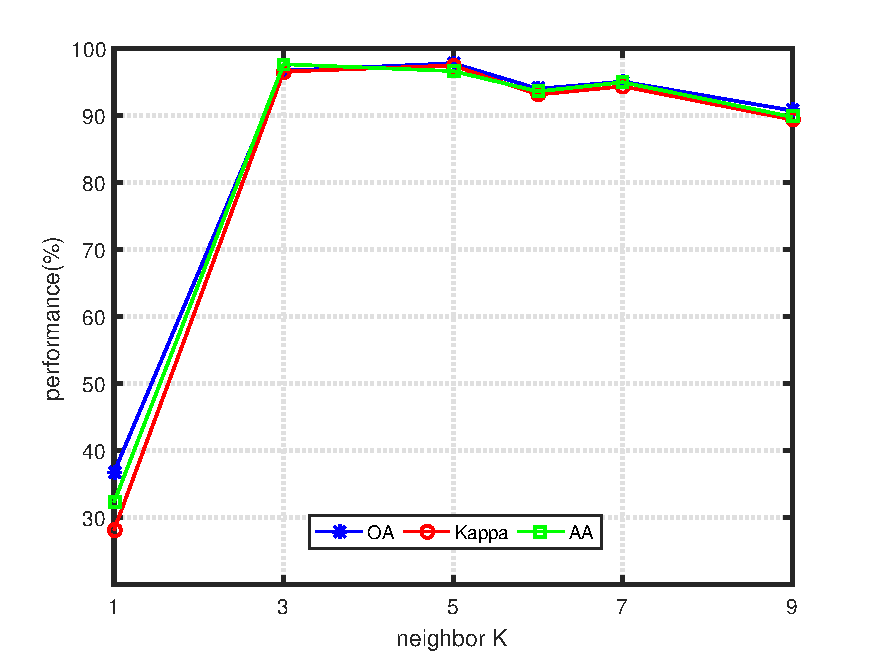
\includegraphics[width=5cm]{image/indianPines_K}}
%\vspace*{8pt}
%\caption{The impact of parameter $K_{nei}$ for Indian Pines.}
%\label{figure3}
%\end{figure*}
%
%\begin{figure*}[bh]
%\centerline{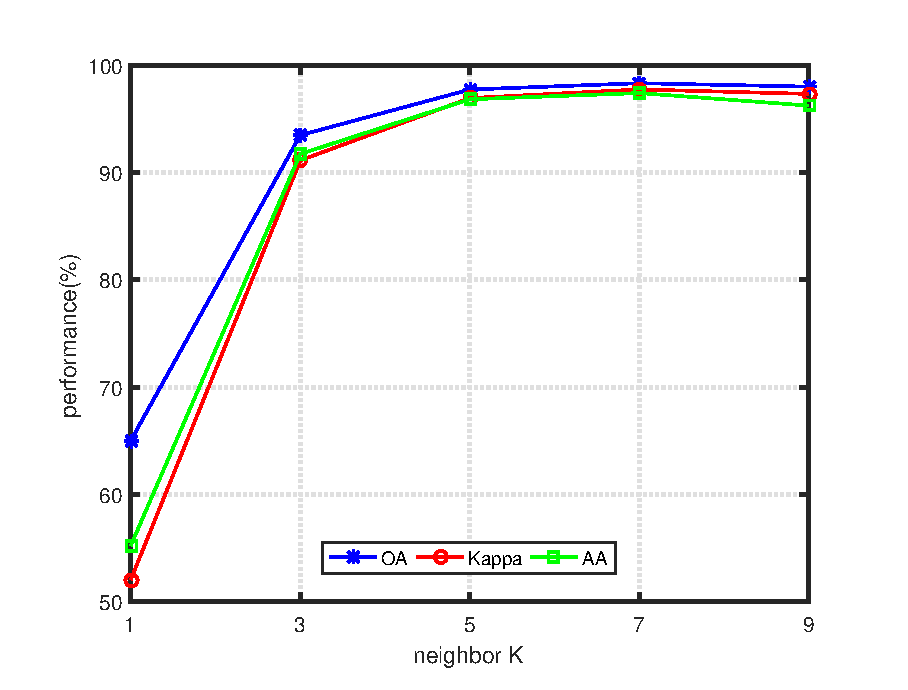
\includegraphics[width=5cm]{image/paviaU_K}}
%\vspace*{8pt}
%\caption{The impact of parameter $K_{nei}$ for PaviaU.}
%\label{figure4}
%\end{figure*}



\section{Experiments}\label{sec:experiment}
\subsection{Experimental Design}



In this section, we demonstrate the performance of our proposed method using two real word HSI data sets: Indian Pines and University of Pavia (PaviaU). 
The following methods are implemented and evaluated:
SVM \cite{37}, 3-D wavelet \cite{29}, 3-D Gabor \cite{38}, SVM-3DG \cite{40}, Res. Conv-Deconv Net \cite{41}. 
%For fairness, other methods are carried out to compare with our proposed method:
To be fair, the best performance of all methods are reported in this document.
To be specific, SVM with 5-fold cross-validation is implemented.
For the 3-D Gabor method, the size of filter is 7 $\times$ 7 $\times$ 7.
For the 3-D wavelet method, the size of filter is 2, where Haar wavelet is applied. 
In all experiments, 10\% samples are used for training, and the remaining 90\% ones are used for test. 
%All the experiments are performed on windows system desktop PC with Inter(R) Core(TM) i5-7400 CPU at 3.00GHz, 64bit system, and 8.00 GB RAM. And the MATLAB language is adopted.


\subsubsection{Data Sets}

\begin{figure}[htb]
	\centerline{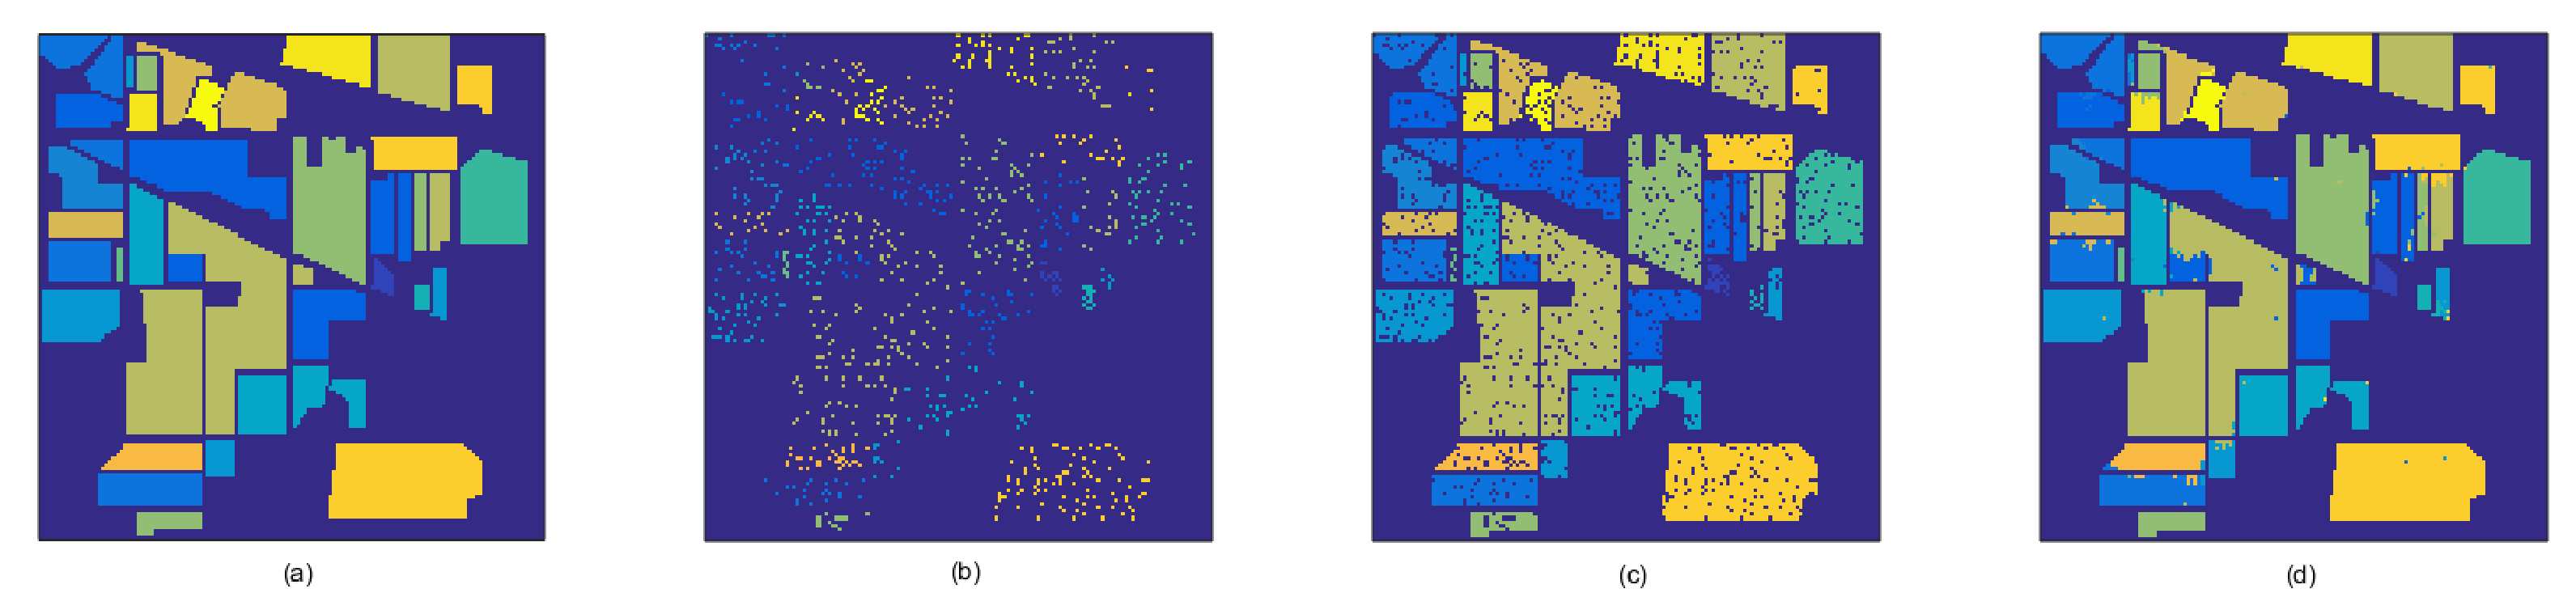
\includegraphics[width=13cm]{image/indian_map}}
	%\vspace*{8pt}
	\caption{Classification maps of Indian Pines scene. (a) Ground truth (b) Training set (c) Test set (d) WTSO (OA=97.75\%)}
	\label{figure7}
\end{figure}


\begin{figure}[bh]
	\centerline{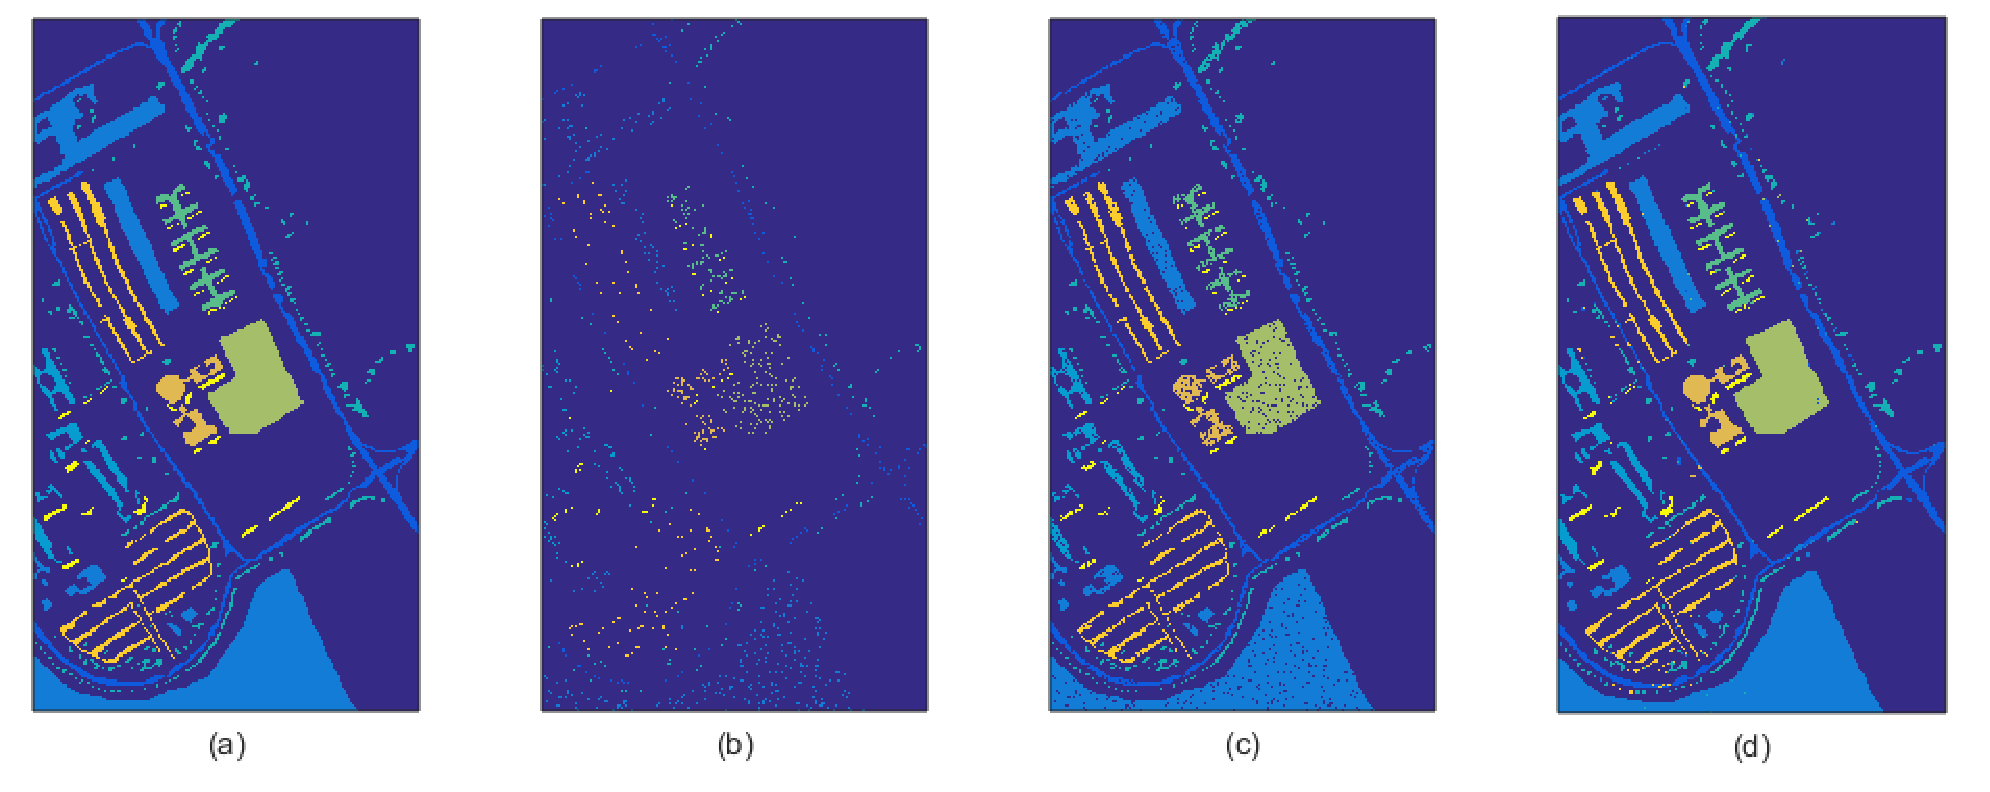
\includegraphics[width=12cm]{image/paviaMap}}
	%\vspace*{8pt}
	\caption{Classification maps of University of Pavia scene. (a) Ground truth (b) Training set (c) Test set (d) WTSO (OA=97.76\%)}
	\label{figure8}
\end{figure}


\begin{itemlist}
 \item The first data set is the Indian Pines which is captured by AVIRIS sensor over the northwestern Indian Pines test site. The size of this data set is 145 $\times$ 145, and it consists of 224 spectral with in the wavelength from $0.4 \times 10^{-6}$ to $0.6 \times 10^{-6}$m. In this scene, the water absorption bands ([104-108],[150-163],220) are removed. There are approximate 10249 labeled pixels with 16 classes. The ground truth of Indian Pines is shown in Fig.~\ref{figure7}(a), where the numbers used for training and test are shown in Table 1.
 
 \item The second data set used in our experiments is University of Pavia, which is gathered by the Reflective Optics System Imaging Spectrometer (ROSIS-03) in Pavia, northern Italy. It contains 115 bands, and the size is 610 $\times$ 340, along with 9 classes. The  spectral coverage ranges from 0.43$\mu$m to 0.86 $\mu$m. The ground truth is shown in Fig.~\ref{figure8}(a), where the numbers of each class used for training and test are shown in Table 2.

\end{itemlist}
\begin{table}[ht]
\tbl{The numbers of training and test samples for University of Pavia.}
{\begin{tabular}{@{}cccc@{}} \toprule
ID & Class name & Train &\ Test \\
  \colrule
 1 & Asphalt & 552 & 6079 \\
             2 & Meadows	& 1160 & 17489 \\
             3 & Gravel	& 303 & 1796 \\
             4 & Trees & 327 & 2737 \\
             5 & Painted metal sheets	 & 260 & 1085 \\
             6 & Bare Soil	 & 439 & 4590 \\
             7 & Bitumen	 & 262 & 1068 \\
             8 & Self-Blocking Bricks	 & 378 & 3304 \\
             9 & Shadows & 231 & 716  \\ \botrule
\end{tabular}}
\label{table2}
\end{table}

\subsubsection{Performance Metrics }

%In a general sense, metric is used to measure the performance of each classes classified correctly.
The results are measured by overall accuracy (OA), average accuracy (AA), and Kappa coefficient (Kappa). In details, OA is the ratio of those correctly classified samples to the total samples. AA is the average of all classes. 
Finally, Kappa coefficient describes the agreement of correct percent classification by performing a random classification test, in which the percentage accuracy is ignored.

\subsection{Experimental Results}
\begin{enumerate}
\item Indian Pines data set. 
%The first data set is Indian Pines. The number of samples is about 1024, which is approximately 10\% of all labeled samples. And remain 90\% samples are used for testing. (removed becaused of the same description as above)
Table 3 shows the classification results of Indian Pines scene of all baseline methods. One can observe that the proposed WTSO obtains the best results in all metrics. 
The OA obtained by 3-D Gabor and WTSO exceeds 90\%, yet the proposed WTSO produces an OA value that exceeds 3-D Gabor by 4.33\%, which is the best. 
For Alfalfa, Corn-notill, Corn, Soybean-mintill and Woods classes, the proposed WTSO obtains the best results. Moreover, Res.Conv-Deconv Net produces the best results in Corn-mintill, Grass-pasture, Grass-trees, Soybean-notill, Wheat, Buildings-Grass-Trees-Drives and Stone-Steel-Towers classes. 
In all, comparing with the results of other baseline methods, the results produced by our WTSO are significantly improved.


\item University of Pavia (PaviaU) data set. In this experiment, we randomly chose 3912 labeled samples, where the ratio is about 8.2\% of all samples. Table 4 shows the classification accuracy of the proposed method when compared with other methods. 
It can be observed that our proposed method produces the best results in OA, whereas 3-D Gabor obtains the best results in AA and Kappa agreement. 
Particularly, WTSO obtains the best performance in Gravel, Bitumen and Self-Blocking Bricks classes. However, the 3-D wavelet method produces the best result in Painted metal sheets class (100\%). Res.Conv-Deconv Net produces the worst results, due to the complexity of neural network.
\end{enumerate}
%Table 3 shows the classification results of Indian Pines scene using our proposed method and the methods being compared. The best results are marked bold. It is obvious that the proposed method produced the best classification accuracy of all OA, AA, and Kappa. Table 4 shown the classification accuracy of the proposed method compared with other approaches for University of Pavia, we can see that the proposed method yielded the best result in metric criterion OA. 3-D Gabor achieved the best accuracy in metric criterion AA and Kappa. Fig.~\ref{figure7} (d) is the classification map using WTSO for Indian Pines scene.  Fig.~\ref{figure8} (d) shown the classification map for PaviaU using proposed method WTSO.

\begin{table}[ht]
\tbl{Classification accuracy (\%) for Indian Pines using different methods. Best results are marked bold. }
{\begin{tabular}{@{}ccccccc@{}} \toprule
Class & SVM  & 3-D wavelet & 3-D Gabor& SVM-3DG &Res.Conv-Deconv Net&\ WTSO \\
  \colrule
1 & 89.29  & 61.22 & 82.65 & 96.77 & 74.86&  \textBF {100.00} \\
2 & 69.92  & 85.33 & 93.60 & 58.46 &95.28 & \textBF {97.85}\\
3 & 57.78 & 80.70 & 90.33 & 93.37 &\textBF{100.00} & 95.60 \\
4 & 71.43  & 54.27 & 92.04 & 96.40 & 95.08& \textBF{98.50} \\
5 & 90.39  & 94.57 & 91.58 & 86.11 & \textBF {96.56} & 95.51 \\
6 & 94.52  & 95.05 & 92.31 & 95.80 &\textBF{99.09} & 97.89 \\
7 & 85.71  & 55.83 & 72.92 & \textBF{100.00} & 84.42 &\textBF{100.00} \\
8 & 96.98  & 97.65 & 99.37 & \textBF {100.00} &74.57 & 99.77 \\
9 &  88.89  & 55.79  &61.05 &  \textBF{100.00} &80.14 & 80.00 \\
10 & 75.17  & 80.27 & 90.03 & 68.86 & \textBF{100.00} & 97.76 \\
11 & 84.57  & 86.30 & 95.51 & 78.57 & 95.74 &\textBF{98.66} \\
12 & 74.95  & 82.06 & 85.74 & \textBF{96.89} &96.06 & 92.57 \\
13 &  97.16  & 95.76 &90.16  &94.21 &\textBF{100.00} &  96.57 \\
14 & 96.62  & 92.95 & 98.58 & 77.84 & 84.62 &\textBF{99.31} \\
15 & 54.94  & 55.22 & 95.19 & 95.42 &\textBF{100.00} & 99.71 \\
16 & 93.65  & 80.70 & 87.33 &  98.72 & \textBF{100.00} & 95.52 \\
\colrule
AA & 83.83  & 78.35 & 88.65 & 89.94 &92.28 &\textBF{96.58} \\
OA & 80.74  & 85.31 & 93.42 & 81.12 &85.76 &\textBF{97.75} \\
Kappa & 78.03  & 83.25 & 92.50 & 78.64 &83.85 &\textBF{97.42} \\
\botrule
\end{tabular}}
\end{table}





%\begin{figure}[bh]
%\centerline{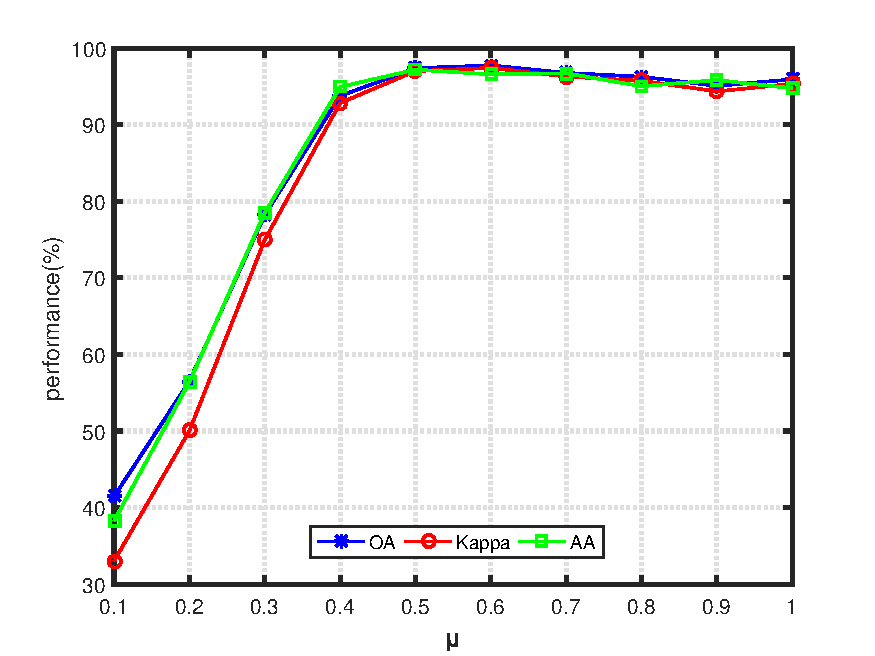
\includegraphics[width=8cm]{image/IndianPines_miu}}
%\vspace*{8pt}
%\caption{The impact of parameter $\mu$ for Indian Pines.}
%\label{figure5}
%\end{figure}
%
%\begin{figure}[bh]
%\centerline{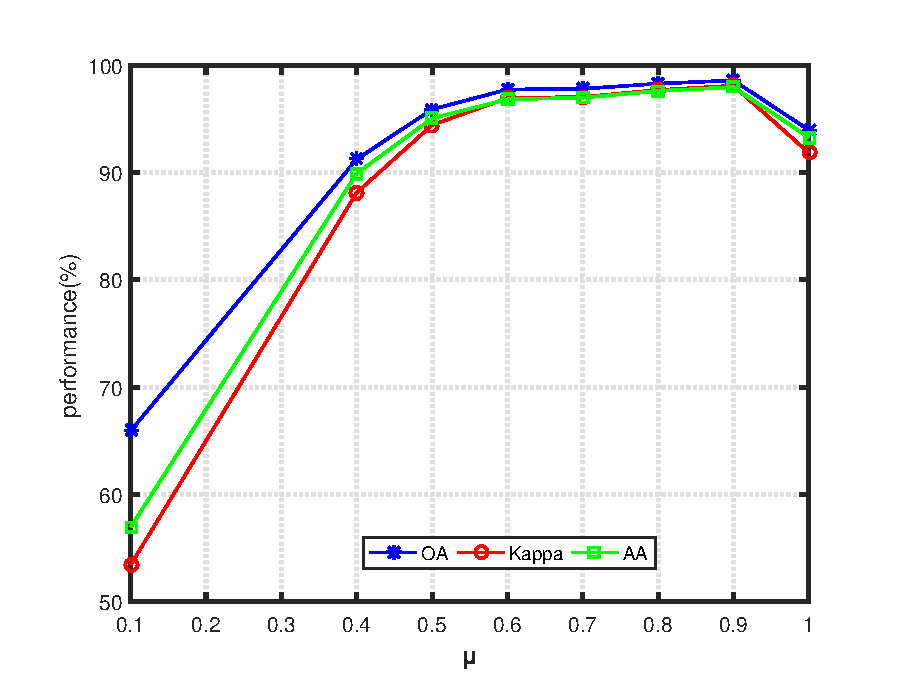
\includegraphics[width=8cm]{image/paviaU_miu}}
%\vspace*{8pt}
%\caption{The impact of parameter $\mu$ for PaviaU.}
%\label{figure6}
%\end{figure}






%\begin{figure}[bh]
%\centerline{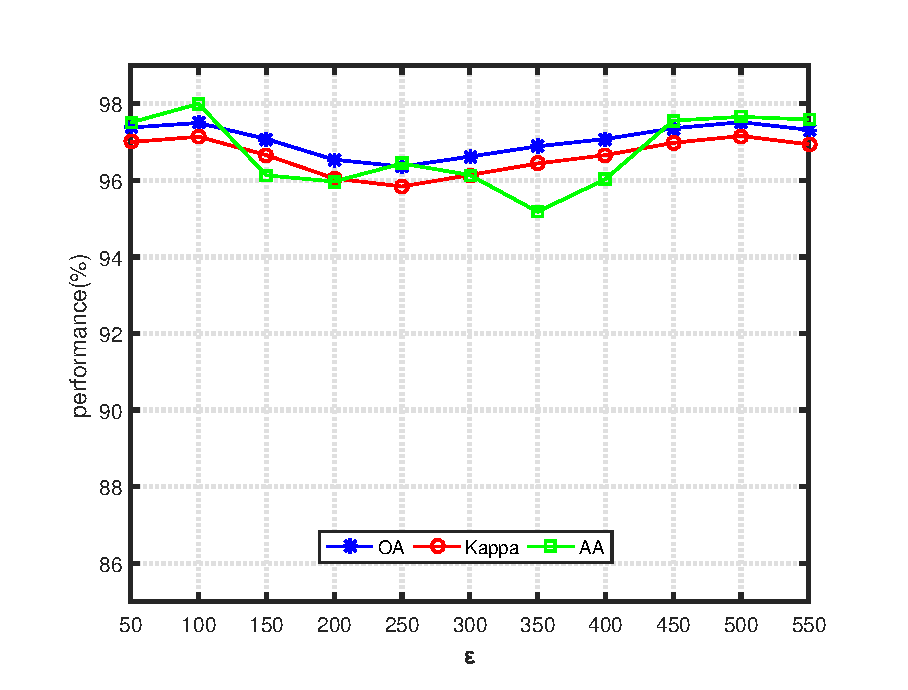
\includegraphics[width=8cm]{image/indianPines_emsou}}
%\vspace*{8pt}
%\caption{The impact of parameter $\epsilon$ for Indian Pines.}
%\label{figure7}
%\end{figure}
%
%
%\begin{figure}[bh]
%\centerline{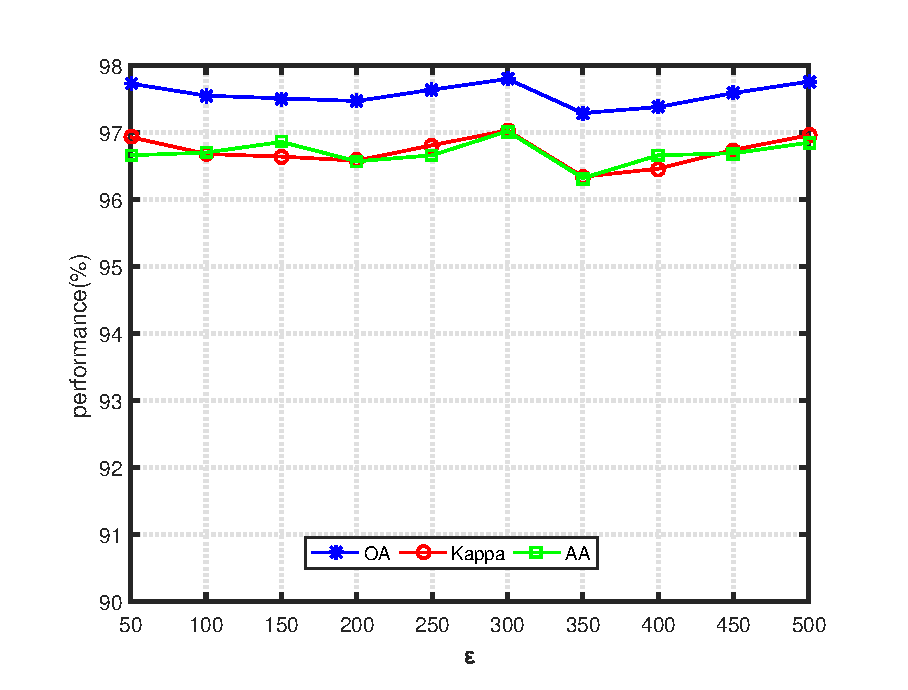
\includegraphics[width=8cm]{image/paviaU_emsou}}
%\vspace*{8pt}
%\caption{The impact of parameter $\epsilon$ for PaviaU.}
%\label{figure8}
%\end{figure}






\begin{table}[ht]
%\sisetup{detect-weight,mode=text}
%\renewrobustcmd{\bfseries}{\fontseries{b}\selectfont}
%\renewrobustcmd{\boldmath}{}
\tbl{Classification accuracy (\%) for University of Pavia using different methods. Best results are marked bold. }
{\begin{tabular}{@{}ccccccc@{}} \toprule
Class & SVM  & 3-D wavelet & 3-D Gabor&SVM-3DG &Res.Conv-Deconv Net&\ WTSO \\
  \colrule
1 & 92.40  & 97.18 & \textBF{98.48} & 97.39 &78.99 & 96.00 \\
2 & 97.83  & 97.64 & \textBF{99.78} &  97.27 &97.16 &99.56 \\
3 & 87.44  & 89.44 & 93.62 &  89.41 &61.46 &\textBF{99.67} \\
4 & 96.03  & 95.73 &  96.42 & \textBF{97.25}  &95.76 &85.23 \\
5 & 99.72  & \textBF{100.00} & 99.18 & 99.61 &97.77 & 99.82 \\
6 & 91.00  & 89.23 & \textBF{99.60} & 98.41 &59.46 &99.23 \\
7 & 90.20  & 93.45 & 90.49 & 98.20  &79.50&\textBF{99.72} \\
8 & 86.94  & 93.42 & 95.88 & 84.00  &96.82&\textBF{98.00} \\
9 &  99.86  & 99.09 & 82.22 &  \textBF{99.89} &92.40&94.40 \\
\colrule
AA & 93.59  & 95.02 & \textBF{97.98} & 95.71 &84.37 & 96.85 \\
OA & 94.32  & 95.65 & 95.07 & 96.06 &87.39 &\textBF{97.76} \\
Kappa & 92.37  & 94.23 & \textBF{97.32} & 94.78 &83.08 &96.96 \\
\botrule
\end{tabular}}

\end{table}


\subsection{Impact of Free Parameters}
Now, we analyze the impact of three free parameters on the classification performance in the proposed WTSO method. Three different experiments are designed on two HSI scenes to evaluate the impact of the free parameters. The final values of these parameters are selected based on the highest score criterion.

\begin{romanlist}[(ii)]
\item Firstly, we analyze the influence of $K_{nn}$ in Eq.~\ref{equ2.7}.
\item Secondly, we discuss the impact of  $\mu$ in Eq.~\ref{equ2.8}. The spatial parameter is very important for the proposed method.
\item In the third experiment, we analyze the effect of  $\epsilon$ in Eq.~\ref{equ2.17}.
\item  In the fourth experiment, the decomposition level of wavelet transform is studied.
\end{romanlist}
\begin{figure*}[bh]
        \centering
        \begin{minipage}[b]{0.45\linewidth}
            \centering
            \centerline{
            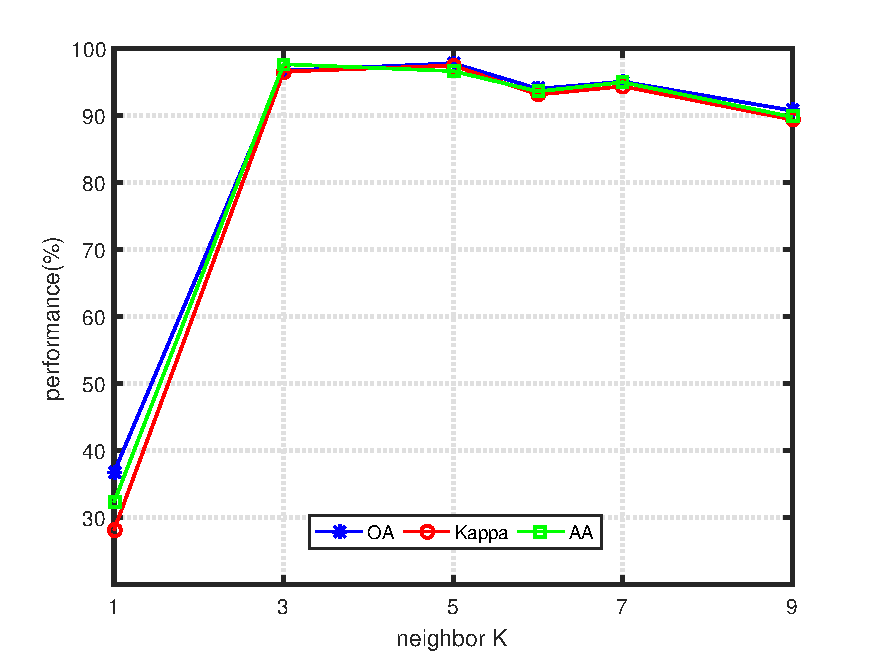
\includegraphics[width=5cm ]{image/indianPines_K}}
            %\includegraphics[width=1.5in]{./Image/PaviaUspectralonly.png}
            \centerline{(a)}
            \medskip
        \end{minipage}
        \begin{minipage}[b]{0.45\linewidth}
            \centering
            \centerline{
            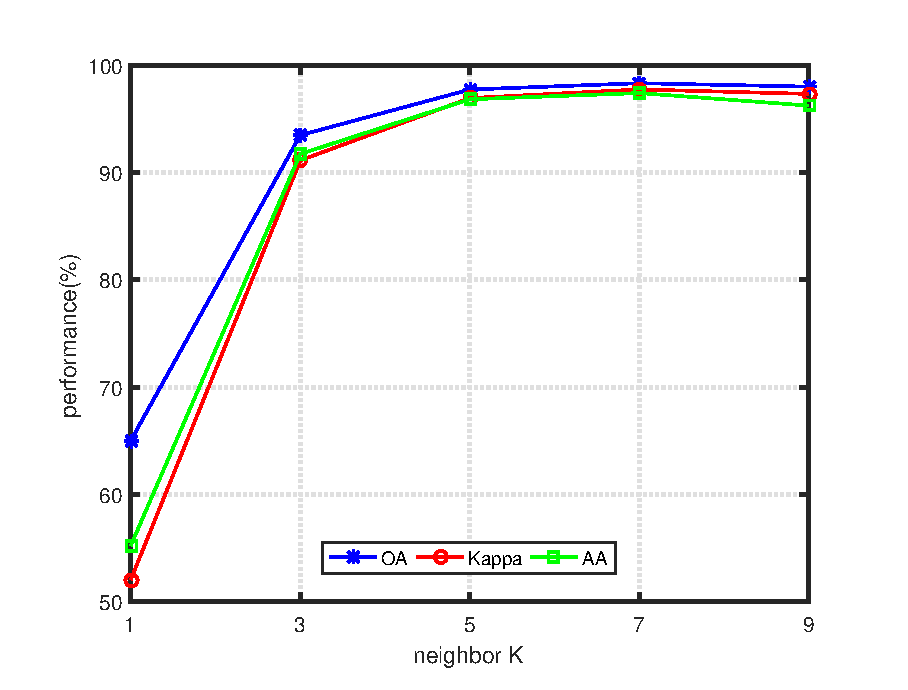
\includegraphics[width=5cm ]{image/paviaU_K}}
            %\includegraphics[width=1.5in]{./Image/PaviaUspectralonly.png}
            \centerline{(b)}
            \medskip
        \end{minipage}
        \caption{The impact of $K_{nn}$. (a) Indian Pines  (b) PaviaU}
        \label{figure3}
    \end{figure*}

Firstly, we discuss the impact of $K_{nn}$ in Eq.~\ref{equ2.7}. We step its value from 1 to 9 using the size of 2. Fig.~\ref{figure3} (a) and Fig.~\ref{figure3}(b) display the impact of $K_{nn}$ for Indian Pines and PaviaU, respectively. 
It can be observed that, for Indian Pines, when $K_{nn}$ ranges from 1 to 3, the performance is sharply increased. 
When $K_{nn}$ rises from 5 to 7, the obtained OA is maximum. When $K_{nn}$ is greater than 7, the classification accuracy is declined. 
For PaviaU, When $K_{nn}$ ranges from 1 to 7, the OA value is increased from 65\% to 98\%, but when $K_{nn}=9$, the OA value is lower than the one when $K_{nn}=7$. 
For Indian Pines, when $K_{nn} = 5$, the highest accuracy is achieved. For PaviaU in Fig.~\ref{figure3}(b), when $1 \leqslant  K_{nn} \leqslant 7$, the result is increasing and the best accuracy is obtained when $K_{nn}=7$.
%ut almost the same as when $K_{nn} = 5$. 
%When $K_{nn}>7$, the performance become smooth. 
Hence, in this paper, based on the above analysis, we use a fixed value in WTSO: $K_{nn}=5$.
\begin{figure*}[bh]
        \centering
        \begin{minipage}[b]{0.45\linewidth}
            \centering
            \centerline{
            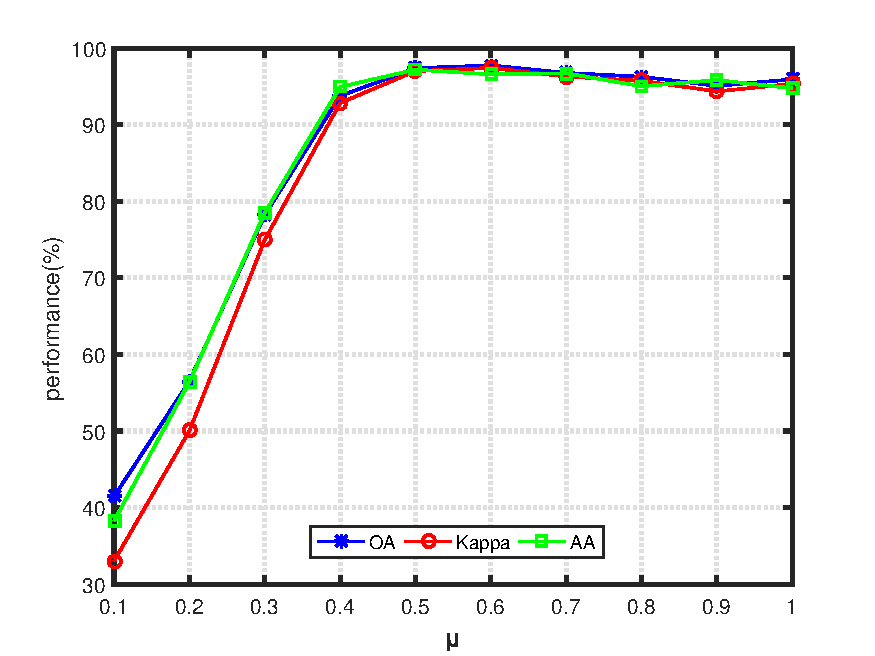
\includegraphics[width=5cm ]{image/IndianPines_miu}}
            %\includegraphics[width=1.5in]{./Image/PaviaUspectralonly.png}
            \centerline{(a)}
            \medskip
        \end{minipage}
        \begin{minipage}[b]{0.45\linewidth}
            \centering
            \centerline{
            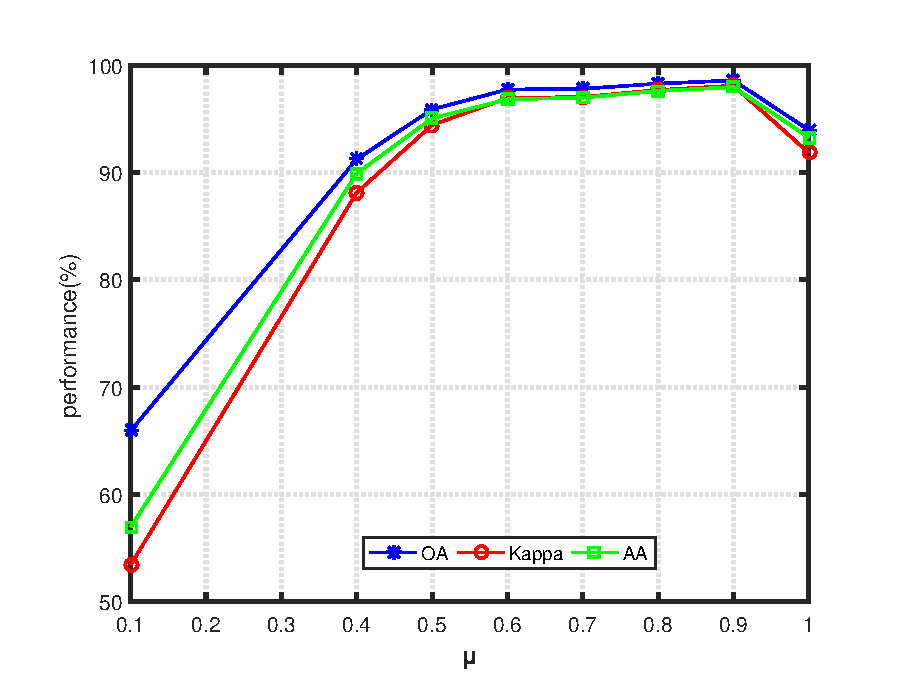
\includegraphics[width=5cm ]{image/paviaU_miu}}
            %\includegraphics[width=1.5in]{./Image/PaviaUspectralonly.png}
            \centerline{(b)}
            \medskip
        \end{minipage}
        \caption{The impact of parameter $\mu$. (a) Indian Pines  (b) PaviaU}
        \label{figure4}
    \end{figure*}

      \begin{figure*}[bh]
        \centering
        \begin{minipage}[b]{0.45\linewidth}
            \centering
            \centerline{
            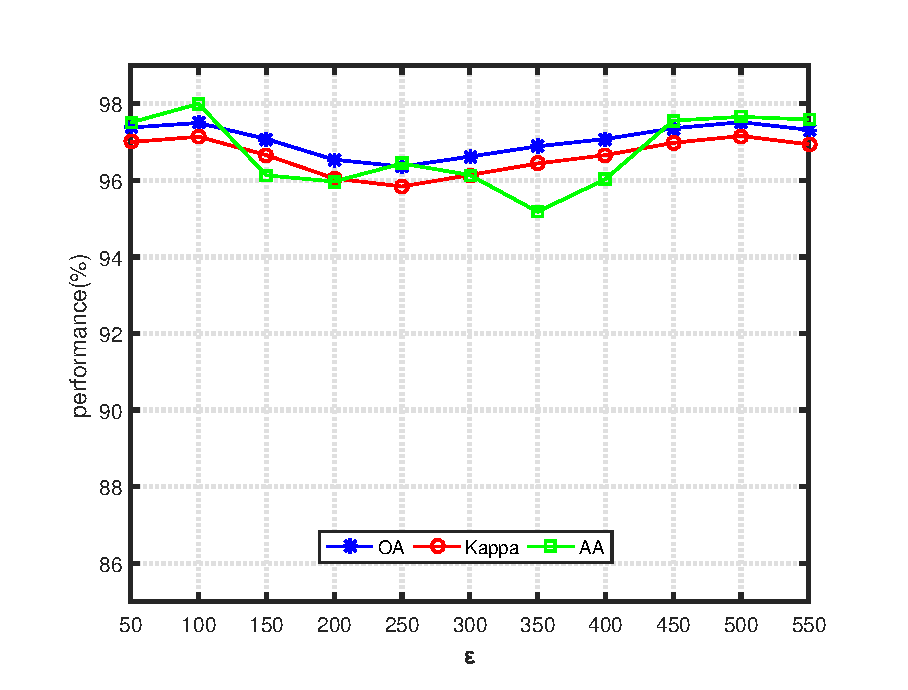
\includegraphics[width=5cm ]{image/indianPines_emsou}}
            %\includegraphics[width=1.5in]{./Image/PaviaUspectralonly.png}
            \centerline{(a)}
            \medskip
        \end{minipage}
        \begin{minipage}[b]{0.45\linewidth}
            \centering
            \centerline{
            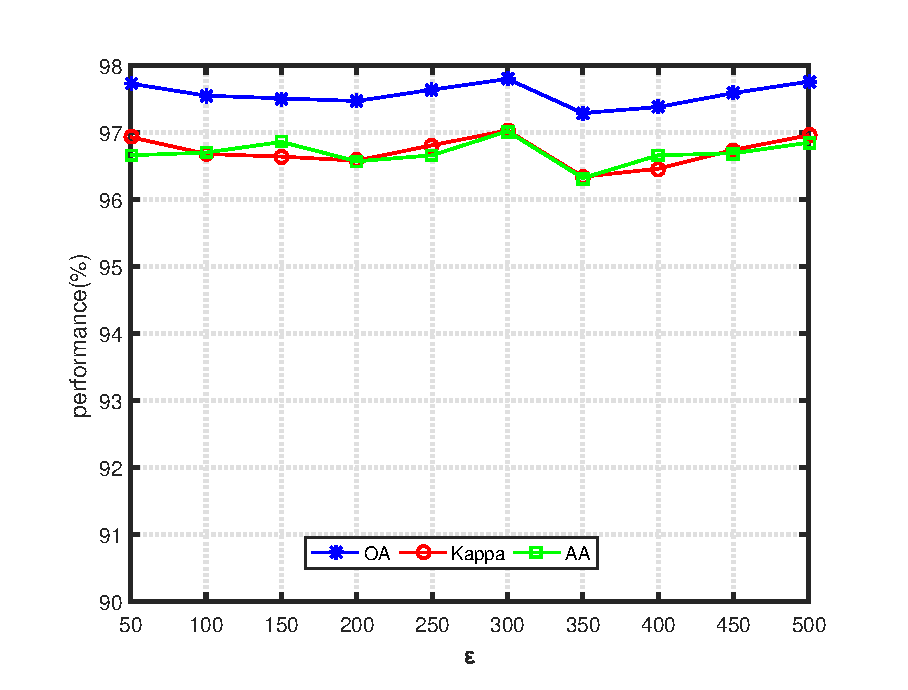
\includegraphics[width=5cm ]{image/paviaU_emsou}}
            %\includegraphics[width=1.5in]{./Image/PaviaUspectralonly.png}
            \centerline{(b)}
            \medskip
        \end{minipage}
        \caption{The impact of parameter $\epsilon$. (a) Indian Pines  (b) PaviaU}
        \label{figure5}
    \end{figure*}

Secondly, the parameter $\mu$ used in Eq.~\ref{equ2.8}, whose role is to balance the spectral information and spatial prior, is very important. 
Fig.~\ref{figure4} (a) and Fig.~\ref{figure4} (b) show the OA, AA and Kappa coefficient when $\mu$ rises from 0.1 to 1, respectively. 
For Indian Pines, when $\mu$ is in the range of [0.1,0.6], the OA, AA, and Kappa coefficient are increased. However, when $\mu$ rises from 0.7 to 1, all of OA, AA, Kappa are declined. Particularly, when $\mu = 0.6$, the performance reaches the maximum for all metrics. 
For PaviaU, when $\mu$ rises from 0.1 to 0.9, the accuracy is increased, and it reaches the maximum value when $\mu=0.9$(OA = 98.61\%, Kappa = 98.12\%, AA = 97.98\%). However, when $\mu = 0.9$, the accuracy is almost the same as $\mu = 0.6$. When $\mu>0.9$, the classification accuracy is decreased. Therefore, for computationally, we choose $\mu$ to be equal to 0.6 in this paper.



  \begin{figure}[htb]
\centerline{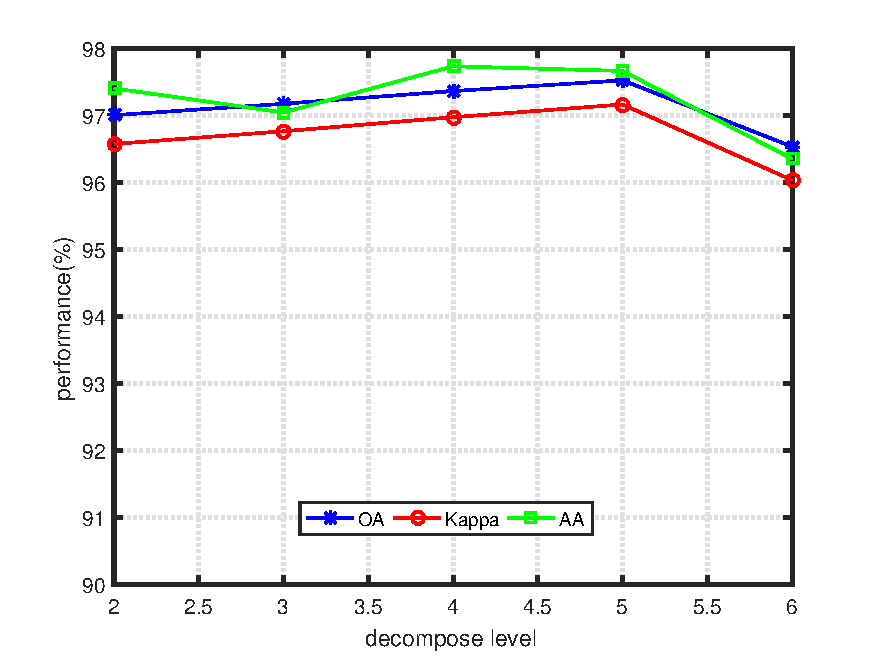
\includegraphics[width=8cm]{image/decomposeLevel}}
\vspace*{8pt}
\caption{The impact of decompose level for Indian Pines.}
\label{figure6}
\end{figure}





In the third experiment, we show the influence of $\epsilon$ in Eq.~\ref{equ2.17} by ranging it from 50 to 550 for Indian Pines, and 50 to 500 for PaviaU, with the step 50 for both images. Fig.~\ref{figure5}(a) and Fig.~\ref{figure5}(b) show the  impact for Indian Pines and PaviaU, respectively. From Fig.~\ref{figure5}(a), we can see that when $\epsilon$ is increased from 50 to 200, all of OA, AA, Kappa are declined for Indian Pines.
However, when it ranges from 250 to 500, the classification accuracy is overall increased (AA is an exception in the rang of 250 to 350). 
When $\epsilon$ is in the range of [350,500], all  metrics are increased, where the best result is obtained when $\epsilon = 500$.
%The is 97.52\% for OA, 97.16\% for Kappa and 97.66\% for AA. 
When $\epsilon>500$, the accuracy becomes smooth and decreasing. In Fig.~\ref{figure5}(b), we can observe that all of AA, OA, Kappa are smooth when $\epsilon$ ranges from 50 to 300.
However, when $\epsilon$ ranges from 300 to 350, all of OA, AA, Kappa are declined. 
And when $\epsilon$ rises from 350 to 500, all of AA, OA, Kappa are increased again.
The highest accuracy is obtained when $\epsilon =500$. Therefore, we choose $\epsilon=500$  in this paper.





Finally, in the fourth experiment, we analyze the impact of decomposition level using Indian Pines, where the level ranges from 2 to 6. 
Fig.~\ref{figure6} shows the results. It is obvious that when increasing the decomposition level from 2 to 5, OA and Kappa are improved, and AA is decreasing when in the range of [2, 3]. 
The best results are obtained when the decomposition level is 5 except AA. However, when the decomposition level is greater than 5, all of AA, OA and Kappa are sharply declined. Hence, we choose the decomposition level to be 5 in this paper.




%
%Fig.~\ref{figure10} and Fig.~\ref{figure11} shown the classification maps for Indian Pines scene and University of Pavia scene respectively. Fig.~\ref{figure10}(a)
%
%It is obviously see that our method obtained smoothly map.




\section{Conclusion}\label{sec:conclude}

%In this paper, a novel method name WTSO is proposed for HSI classification task. This approach is based on wavelet transform and smooth ordering, which is performance effectively in image processing. First, we apply wavelet transform to the image, obtained approximate coefficient. Then, by using smooth ordering among approximate coefficient, which produces a 1D embedding and it in 1D space. Hence, simple 1D processing tool is applied to task. Finally, interpolation is used to build finally classifier for HSI classification task. Experiments demonstrated that the proposed method obtained state of the art result in Indian Pines and best overall accuracy (OA) in University of Pavia. Therefore, the proposed method is effective and promising for HSI classification. In the future work, WTSO can be applied to other signal analysis tools, such as sparse representation.%
A novel and effective method WTSO is proposed for HSI classification in this paper. In the WTSO method, the wavelet transform is first applied to the input signal so that the signal can be decomposed into ACs and DCs. Then, a new distance measurement is applied before smooth ordering to obtain the similarity of different samples. 
%Based the smooth ordering, in WTSO, 
The obtained ACs are smoothly embedded onto a 1-D space, after that, the simple 1-D tools, such as interpolation, can be used for constructing the candidate classifiers. 
%Finally, the classifier is established using interpolation. 
And the final classifier are constructed using multiple 1-D embeddings.
The WTSO method processes ACs in low-dimensional space, which is more explicit. To demonstrate the effectiveness of WTSO, two real HSI data sets are experimentally evaluated. Compared with other recently proposed state-of-the-art wavelet-based methods, our approach can obtain higher accuracy in most cases.

\section{Acknowledgement}
This work was supported by the National Natural Science Foundation with No. 61862005, and Natural Science Foundation of Guangxi with No. 2017GXNSFBA198226.
This work was also supported by National Key R\&D Program of China under Grant 2017YFA0700800.

%This work was financially supported by the Guangxi Natural Science Foundation No.2017GXNSFBA198226, Scientific Research Foundation of Guangxi University No.XGZ160483, and by the Higher Education undergraduate Teaching Reform project of Guangxi with No.2017JGB108, it also supported by the project with No. DD3070051008.



\bibliographystyle{ws-ijwmip}
\bibliography{RefBibData}

\end{document}

